% \documentclass[11pt,a4paper]{article}

% \usepackage[margin=2.3cm]{geometry}
% \usepackage[T1]{fontenc}
% \usepackage{lmodern}
% \usepackage{microtype}
% \usepackage{graphicx}
% \usepackage{booktabs}
% \usepackage{xcolor}
% \usepackage{amsmath}
% \usepackage{caption}
% \usepackage{float}
% \usepackage{tikz}
% \usetikzlibrary{shapes,arrows.meta,positioning}
% \usepackage{pgfplots}
% \pgfplotsset{compat=1.16}
% \usepackage[hidelinks]{hyperref}

% \captionsetup{font=small,labelfont=bf}
% \setlength{\parskip}{3pt}
% \setlength{\parindent}{0pt}

% % ---- helpers -------------------------------------------------------------
% \newcommand{\todo}[1]{\textcolor{red}{[TODO: #1]}}
% % \figimg{file}{width}: includes the image if it exists, otherwise draws an empty box
% \newcommand{\figimg}[2]{%
%   \IfFileExists{#1}{\includegraphics[width=#2]{#1}}%
%   {\fbox{\parbox[c][5cm][c]{#2}{\centering\small\texttt{MISSING: #1}}}}}
% \newcommand{\gene}[1]{\textit{#1}}

% \title{\vspace{-1.2cm}\textbf{Direct and indirect links between microglial genes and Alzheimer's pathology severity:\\
% a comparison of ARACNE, PC and MIIC on SEA-AD data}}
% \author{
%   Mehrdad Hadidian \\
%   \small\texttt{mehrdad.hadidian@etu.sorbonne-universite.fr}
%   \and
%   Pavel Borisenko \\
%   \small\texttt{pavel.borisenko@etu.sorbonne-universite.fr}
%   \\[4pt]
%   \small RESYS course project, Sorbonne Université
% }
% \date{}

% \begin{document}
% \maketitle
% \vspace{-0.8cm}

% \begin{abstract}
% \noindent
% Microglia respond strongly to Alzheimer's disease (AD), but it remains unclear which microglial genes are \emph{directly} associated with pathology severity and which are linked only through other genes. We reconstructed gene networks for 48 microglial genes together with a continuous pathology score (CPS) and a sequencing-depth variable, using three network inference methods (ARACNE, PC and MIIC), on single-nucleus RNA-seq data from the middle temporal gyrus (MTG) of the SEA-AD cohort. We compared two data representations: metacells (sums of 30 nuclei) and single nuclei. The three methods agreed on 21 (metacells) and 18 (nuclei) edges, mostly known biology such as \gene{C1QA}--\gene{C1QB} and \gene{CD74}--\gene{HLA-DRA}. MIIC linked CPS to 19 genes on metacells, but a control with CPS shuffled between donors produced the same $\sim$18 links, showing that they are a donor-level artefact. After this control, \gene{PTPRG}, a marker of the disease-associated microglia (DAM) state, was the only robust CPS neighbour across all three methods. Our results illustrate that metacell aggregation can create spurious links to donor-level variables, and that shuffling controls are essential for such analyses.
% \end{abstract}

% % =========================================================================
% \section{Introduction}
% Alzheimer's disease is characterised by amyloid plaques and tau tangles, and by a prominent response of the brain's immune cells, the microglia. Genome-wide association studies have identified many AD risk genes that are expressed predominantly in microglia, including \gene{TREM2}, \gene{PLCG2}, \gene{INPP5D}, \gene{CD33} and \gene{MS4A6A}~\cite{Gabitto2024}. Single-nucleus RNA sequencing (snRNA-seq) allows one to study how microglial states change with disease. The Seattle Alzheimer's Disease Brain Cell Atlas (SEA-AD) profiled the middle temporal gyrus (MTG) of 84 donors and defined a continuous pseudo-progression score (CPS) that orders donors along the pathological trajectory~\cite{Gabitto2024,Hawrylycz2024}. Gabitto et al.\ showed that the proportion of a disease-associated microglial supertype (Micro-PVM\_3) increases with CPS, and identified genes that change early or late along this trajectory. An independent analysis of the same data using hdWGCNA on metacells described microglial co-expression modules, but with disease as discrete groups and without explicit gene--gene edges~\cite{Adeoye2025}.

% Co-expression and differential expression analyses do not distinguish a \emph{direct} relation between a gene and the disease from an \emph{indirect} one, mediated by other genes. This is the question addressed by network reconstruction: if two variables become independent once a third (or a set of others) is known, the edge between them is removed. Several families of methods exist. ARACNE is an information-theoretic method that prunes indirect edges using the data processing inequality~\cite{Margolin2006}. The PC algorithm is a constraint-based causal discovery method based on conditional independence tests~\cite{Spirtes2000}. MIIC is also constraint-based but uses an information-theoretic criterion to detect and orient edges, accepts mixed (continuous and discrete) data and can flag possible latent common causes~\cite{Verny2017,Cabeli2020}. The methods rely on different assumptions, so edges found by all three are more trustworthy.

% \textbf{Goal.} We asked (i) which microglial genes are directly linked to CPS and which only through other genes, and (ii) how well ARACNE, PC and MIIC agree. A second, methodological goal emerged during the project: to determine how data representation (metacells versus single nuclei) influences the networks, especially for a variable such as CPS which has only one value per donor.

% % =========================================================================
% \section{Materials and methods}
% \subsection{Data and cell selection}
% We used the June 2026 release of the SEA-AD immune-cell dataset (240{,}651 nuclei $\times$ 36{,}601 genes, 84 donors, 10 brain regions). Raw UMI counts (integers) were used throughout; the normalised matrix was not used, except for ranking genes during selection. CPS is not stored in the expression file; we took the regional score \texttt{CPS\_Local} for MTG from the SEA-AD CPS table (0 = almost no pathology, 1 = most severe pathology in the cohort; one value per donor). As a sanity check, median CPS rose with ADNC category (Not AD 0.06, Low 0.14, Intermediate 0.43, High 0.68) and with Braak stage (0.08 to 0.70).

% We kept MTG nuclei, removed monocytes and lymphocytes, and applied quality control, leaving 34{,}679 nuclei from 83 donors. Using marker-gene detection rates we interpreted the supertypes as follows: Micro-PVM\_2 (and its sub-clusters 2\_1, 2\_3) as homeostatic microglia (\gene{P2RY12} detected in 77\% of nuclei), Micro-PVM\_3-SEAAD and Micro-PVM\_4-SEAAD as reactive/DAM states (\gene{GPNMB} 43--49\%; \gene{SPP1} 95\% in PVM\_4), and Micro-PVM\_1 as perivascular macrophages (\gene{MRC1} 73\%, \gene{CD163} 91\%, \gene{P2RY12} 21\%), which we excluded. This agrees with the annotation of Gabitto et al.\ (Fig.~6).

% \subsection{Metacells and single-nucleus data}
% Only a small fraction of the transcripts is captured per nucleus (median $\sim$2{,}600 genes and $\sim$5{,}300 UMIs), so many informative genes are mostly zero (\gene{TREM2} is non-zero in 23\% of nuclei). Network methods search for coordinated changes between rows, and random zeros hide such coordination. Following the metacell idea~\cite{Baran2019,Morabito2023}, we randomly split the nuclei of each donor$\times$supertype pair into groups of 30 and \emph{summed} their raw counts (a sum of integers remains raw counts). This yielded \textbf{983 metacells from 81 donors} (1--32 per donor); \gene{TREM2} is non-zero in 99\% of metacells. Every metacell comes from a single donor, so donors are never mixed.

% Sequencing depth raises all genes simultaneously (gene--depth correlation up to 0.78). Instead of normalising, we added the total UMI count per row as a network variable, \texttt{total\_UMIs}, to absorb depth-driven edges. As an alternative representation (``Experiment B'') we built a dataset with 12 random single nuclei per donor (996 rows), with the same variables.

% \subsection{Gene selection}
% We kept genes non-zero in at least 80\% of metacells and chose 48 genes in two ways (Table~\ref{tab:genes}). Biology-based genes (34) were taken from known homeostatic markers, disease-response genes, AD risk genes and transcription factors. Data-driven genes (14) were those higher in reactive (PVM\_3/4) than in homeostatic (PVM\_2) microglia. A first attempt using the most variable genes returned mostly unannotated non-coding RNAs, stress genes and genes of other cell types or genotype effects, and was discarded; similarly, data-driven ``homeostatic'' genes turned out to be contamination from other cells and were replaced by known markers. \textbf{Genes were not selected by their association with CPS.} The final network has 50 variables: 48 genes, \texttt{CPS\_Local} and \texttt{total\_UMIs}.

% \begin{table}[ht]
% \centering\small
% \caption{Genes included in the network (48 genes + CPS + total UMIs).}\label{tab:genes}
% \begin{tabular}{p{3.2cm}p{12.3cm}}
% \toprule
% Group & Genes \\
% \midrule
% Homeostatic (13) & \gene{P2RY12, P2RY13, CX3CR1, TMEM119, CSF1R, SALL1, GPR34, OLFML3, HEXB, SELPLG, TGFBR1, SLC2A5, CST3}\\
% Disease response (10) & \gene{TREM2, TYROBP, APOE, SPP1, GPNMB, CD74, HLA-DRA, C1QA, C1QB, CD163}\\
% AD risk genes (8) & \gene{PLCG2, INPP5D, MS4A6A, PICALM, SORL1, BIN1, CD33, ABI3}\\
% Transcription factors (3) & \gene{SPI1, IRF8, MEF2C}\\
% Data-driven, reactive (14) & \gene{TPRG1, DIRC3, FAM20A, TGFBI, PLIN2, PTPRG, FGR, CD83, TBC1D2, IQGAP2, GAS2L3, ZNF804A, PLXNC1, CDK14}\\
% \bottomrule
% \end{tabular}
% \end{table}

% \subsection{Network reconstruction methods}
% We applied three methods from the course, chosen because they rest on different principles. \textbf{ARACNE} computes pairwise mutual information and removes the weakest edge of every triangle (data processing inequality); it is fast and robust but undirected. The \textbf{PC algorithm} starts from a complete graph and removes edges using conditional independence tests, then orients edges; it assumes causal sufficiency and is usually tailored to Gaussian or discrete data. \textbf{MIIC} combines a mutual-information-based search for conditional independencies with an orientation step, handles non-linear and non-monotone dependencies, and can mark edges as possibly produced by a latent common cause. A \emph{consensus edge} is an edge present in all three networks. Figure~\ref{fig:pipeline} summarises the workflow.

% \begin{figure}[ht]
% \centering
% \begin{tikzpicture}[node distance=0.55cm and 0.75cm,
%   box/.style={draw,rounded corners,align=center,font=\footnotesize,minimum height=0.95cm,text width=2.35cm},
%   arr/.style={-{Latex[length=2mm]},thick}]
% \node[box] (a) {SEA-AD snRNA-seq\\(raw UMIs)};
% \node[box,right=of a] (b) {MTG microglia\\QC, drop PVM\_1};
% \node[box,right=of b] (c) {metacells (30 nuclei)\\or single nuclei};
% \node[box,right=of c] (d) {48 genes + CPS\\+ total UMIs};
% \node[box,right=of d] (e) {ARACNE, PC, MIIC\\consensus};
% \node[box,below=0.7cm of d] (f) {shuffle CPS\\between donors};
% \draw[arr] (a)--(b); \draw[arr] (b)--(c); \draw[arr] (c)--(d); \draw[arr] (d)--(e);
% \draw[arr] (d)--(f); \draw[arr] (f)-|(e);
% \end{tikzpicture}
% \caption{Overview of the analysis. The shuffling control (CPS permuted between donors) is run on both data representations and its output is compared with the networks obtained with the real CPS.}\label{fig:pipeline}
% \end{figure}

% \subsection{Control for the donor effect}
% CPS has a single value per donor, so in the 983-row metacell table it takes only 81 distinct values and acts as a donor identifier. To separate a true disease association from a donor effect, we repeated the inference with CPS \emph{shuffled between donors}: each donor keeps one value, but that of another person, which destroys the link with disease while preserving the donor-ID structure. On nuclei we used five different samples of 12 nuclei per donor, each with real and shuffled CPS; on metacells we ran two shuffles.

% \subsection{Comparison with the literature}
% We compared our genes with the supertype markers and the genes changing along CPS in Gabitto et al.\ (Fig.~6) and with the hdWGCNA microglial modules MIC-M1 to M5 of Adeoye et al.\ (Fig.~8). Spearman correlations of genes with CPS were computed on normalised metacells for orientation only, as they are overconfident (one CPS value per donor). All analyses were done in R; the code is provided with the report.

% % =========================================================================
% \section{Results}
% \subsection{Network structure and agreement between methods}
% On metacells, ARACNE, PC and MIIC returned 71, \todo{PC edges; recomputed value} and 111 edges, respectively, and on single nuclei 57, \todo{PC} and 84 edges. The three methods agreed on \textbf{21 edges on metacells} and \textbf{18 on nuclei} (Table~\ref{tab:comp}). The PC edge counts in an earlier run were underestimated because of a bug in edge counting (edges set during orientation conflict resolution were lost); the PC numbers and the consensus will be updated after rerunning the pipeline.

% The consensus edges reproduce known biology (Fig.~\ref{fig:miic_meta}): the two chains of the complement complex (\gene{C1QA}--\gene{C1QB}), MHC-II and its chaperone (\gene{CD74}--\gene{HLA-DRA}), homeostatic markers (\gene{P2RY12}--\gene{CX3CR1}, \gene{P2RY12}--\gene{SALL1}, \gene{GPR34}--\gene{OLFML3}), disease-response links (\gene{APOE}--\gene{TYROBP}, \gene{APOE}--\gene{C1QA}), the AD-risk pair \gene{MS4A6A}--\gene{PLCG2}, and links among reactive-state genes (\gene{GPNMB}--\gene{IQGAP2}, \gene{TPRG1}--\gene{ZNF804A}, \gene{CD163}--\gene{TGFBI}/\gene{FGR}). \texttt{total\_UMIs} absorbed the genes most sensitive to depth (\gene{MEF2C}, \gene{PICALM}, \gene{PLCG2}; correlation $\sim$0.75), as intended.

% \begin{figure}[ht]
% \centering
% % >>> PUT: MIIC network on METACELLS (file results/networks/net_miic.png)
% \figimg{figures/net_miic.png}{0.88\linewidth}
% \caption{MIIC network reconstructed on 983 metacells (48 genes, \texttt{CPS\_Local}, \texttt{total\_UMIs}). Edges and orientations as returned by MIIC; \texttt{CPS\_Local} is connected to many genes, which is shown below to be a donor artefact.}\label{fig:miic_meta}
% \end{figure}

% \subsection{Effect of data representation}
% Moving from metacells to single nuclei weakened gene--gene correlations because of zeros (for example \gene{C1QA}--\gene{C1QB}: 0.81 to 0.47), and sparse genes (\gene{OLFML3} in 7\% of nuclei, \gene{GAS2L3} in 8\%) lost their edges. Of the 18 gene--gene consensus edges on metacells, \textbf{6 were also found by all three methods on nuclei}: \gene{APOE}--\gene{C1QA}, \gene{APOE}--\gene{TYROBP}, \gene{CD74}--\gene{HLA-DRA}, \gene{CX3CR1}--\gene{P2RY12}, \gene{GPNMB}--\gene{IQGAP2} and \gene{DIRC3}--\gene{IQGAP2}; five were found by one or two methods and seven disappeared. We regard these six as the most reliable links of the project. Depth effects were larger in nuclei (a 27-fold range of UMIs per nucleus), and the number of \texttt{total\_UMIs} neighbours rose from 12 to 29 for MIIC (Table~\ref{tab:comp}).

% \begin{figure}[ht]
% \centering
% % >>> PUT: MIIC network on SINGLE NUCLEI (file results/networks_nuclei/net_miic.png)
% \figimg{figures/net_miic_nuc.png}{0.88\linewidth}
% \caption{MIIC network reconstructed on single nuclei (12 random nuclei per donor, 996 rows), with the same 50 variables as in Fig.~\ref{fig:miic_meta}. \texttt{CPS\_Local} has only two neighbours here.}\label{fig:miic_nuc}
% \end{figure}

% \begin{table}[ht]
% \centering\small
% \caption{Comparison of the two data representations. PC values marked * come from the run affected by the edge-counting bug and will be updated.}\label{tab:comp}
% \begin{tabular}{lcc}
% \toprule
%  & Metacells & Single nuclei\\
% \midrule
% Edges ARACNE / PC / MIIC & 71 / \todo{PC}* / 111 & 57 / \todo{PC}* / 84\\
% Consensus edges (3 methods) & 21 & 18\\
% CPS neighbours ARACNE / PC / MIIC & 1 / 0* / \textbf{19} & 2 / 2* / 2\\
% MIIC edges flagged as latent common cause & 9 & 0\\
% \texttt{total\_UMIs} neighbours ARACNE / PC / MIIC & 8 / 3* / 12 & 26 / 8* / 29\\
% \bottomrule
% \end{tabular}
% \end{table}

% % \begin{figure}[ht]
% % \centering
% % % >>> OPTIONAL: consensus network on single nuclei (file results/networks_nuclei/net_consensus.png).
% % % If you prefer, use results/networks/net_consensus.png (metacells) or remove this figure.
% % \figimg{figures/consensus_nuclei.png}{0.7\linewidth}
% % \caption{Consensus network on single nuclei: edges found by ARACNE, PC and MIIC simultaneously (18 edges).}\label{fig:cons}
% % \end{figure}

% \subsection{CPS neighbours: donor artefact and robust links}
% On metacells MIIC connected CPS to 19 variables, whereas ARACNE and PC found at most one (Table~\ref{tab:comp}). Many of these genes had almost no correlation with CPS, and six of the edges were flagged as latent common cause. The shuffling control showed why (Fig.~\ref{fig:cps} and Table~\ref{tab:stab}): \textbf{with CPS shuffled between donors, MIIC on metacells still returned 18 neighbours in both repeats} (including \gene{APOE}, \gene{BIN1}, \gene{C1QB}, \gene{CD74}, \gene{CSF1R}, \gene{P2RY12}, \gene{SPP1}), although no link with disease exists by construction. On single nuclei, the shuffled variable gave only 0.2--0.8 neighbours on average, versus 2.2--3.0 for real CPS. Hence the 19 MIIC links on metacells reflect differences between people (genetics, circumstances of death, tissue handling) that metacell aggregation makes very sharp, rather than disease.

% \begin{figure}[ht]
% \centering
% \begin{tikzpicture}
% \begin{axis}[ybar, bar width=7pt, width=0.92\linewidth, height=5.6cm,
%   symbolic x coords={ARACNE,PC,MIIC}, xtick=data,
%   ylabel={mean \# CPS neighbours}, ymin=0, ymax=21,
%   legend style={font=\scriptsize, at={(0.02,0.98)}, anchor=north west, legend columns=2},
%   enlarge x limits=0.25, tick label style={font=\small}, ylabel style={font=\small}]
% \addplot coordinates {(ARACNE,2.2) (PC,3.0) (MIIC,2.6)};
% \addplot coordinates {(ARACNE,0.2) (PC,0.8) (MIIC,0.8)};
% \addplot coordinates {(ARACNE,1) (PC,0) (MIIC,19)};   % TODO: update PC (metacells, real CPS) after fixing the bug
% \addplot coordinates {(ARACNE,2.5) (PC,1.5) (MIIC,18)};
% \legend{Nuclei real CPS, Nuclei shuffled CPS, Metacells real CPS, Metacells shuffled CPS}
% \end{axis}
% \end{tikzpicture}
% \caption{Number of CPS neighbours per method with real and shuffled CPS, for single nuclei (mean over five samples) and metacells. MIIC on metacells finds $\sim$18--19 neighbours with real \emph{and} shuffled CPS. The PC bar for metacells with real CPS comes from the run affected by the edge-counting bug (\todo{update}).}\label{fig:cps}
% \end{figure}

% Over five independent samples of nuclei, a small set of genes remained robustly connected to CPS (Table~\ref{tab:stab}). \textbf{\gene{PTPRG}} was a CPS neighbour in 4/5 (ARACNE), 5/5 (PC) and 5/5 (MIIC) samples and never appeared with shuffled CPS. \gene{IQGAP2} was second (3/5, 4/5, 2/5), and \gene{BIN1} appeared in 2/5 samples with a negative association. \gene{TGFBI}, found by all three methods in the first nucleus sample, appeared in only 1 of 15 runs afterwards and is therefore a sample-specific result. With random CPS, 0--2 spurious neighbours appeared per run (different genes each time), which gives a reference level of false links.

% \begin{table}[ht]
% \centering\small
% \caption{Stability of CPS neighbours over five independent nucleus samples (number of samples in which the gene is a CPS neighbour).}\label{tab:stab}
% \begin{tabular}{lccc}
% \toprule
% Gene & ARACNE & PC & MIIC\\
% \midrule
% \gene{PTPRG} & 4/5 & 5/5 & 5/5\\
% \gene{IQGAP2} & 3/5 & 4/5 & 2/5\\
% \gene{BIN1} (negative) & \multicolumn{3}{c}{2/5 (all methods combined)}\\
% \gene{TGFBI} & \multicolumn{3}{c}{1/15 runs}\\
% \bottomrule
% \end{tabular}
% \end{table}

% \subsection{Agreement with published work}
% \gene{PTPRG}, \gene{TPRG1} and \gene{ZNF804A}, which we selected from the data, are among the DAM-supertype markers of Gabitto et al.\ (Fig.~6c), and in our networks they are connected to each other (\gene{TPRG1}--\gene{ZNF804A} by all methods on metacells; \gene{PTPRG}--\gene{ZNF804A} by ARACNE and MIIC). That \gene{PTPRG} is also our robust CPS neighbour is consistent with the increase of the DAM supertype along CPS. We also reproduced the \gene{APOE}--\gene{CST3} link of the Adeoye MIC-M2 module (ARACNE and MIIC, on both representations). In contrast, early-response genes of Gabitto (\gene{CSF1R}, \gene{C1QA/B}, \gene{IRF1/7}, Fc receptors) hardly correlated with CPS in our data (Spearman $\rho$ from $-0.2$ to $+0.17$). Genes increasing with CPS both in the papers and in our data but absent from our set include \gene{CTSD} ($\rho\approx+0.33$), \gene{NHSL1}, \gene{TANC2}, \gene{CADM1}, \gene{WIPF3}, \gene{MITF}, \gene{STARD13} and \gene{CD81}.

% % =========================================================================
% \section{Discussion}
% \textbf{Which genes are directly linked to pathology?} Only \gene{PTPRG} was a reproducible direct neighbour of CPS across methods and samples; \gene{IQGAP2} and \gene{BIN1} are weaker candidates. This is a modest result, but a credible one: it is consistent with the DAM marker annotation, was never produced by shuffled CPS, and appears with the three methods, which rely on different assumptions. Because \gene{PTPRG} was selected as a data-driven marker of reactive microglia and not by its association with CPS, this finding is not circular. Most other genes (for example \gene{APOE}, \gene{CD74}, \gene{C1QA/B}) are tightly connected to each other, which suggests that their relation to disease is better described as the activity of a state (a reactive programme) than as individual direct effects.

% \textbf{Metacells are a double-edged tool.} Aggregation recovered clean and biologically plausible gene--gene networks that single nuclei could not (many links vanished in nuclei because of zeros). But for a donor-level variable such as CPS, the same aggregation removes within-donor noise and leaves differences between people as the dominant signal. MIIC, which detects any statistical dependence and not only monotone trends, then connects CPS to everything that distinguishes donors. Without the shuffling control we would have reported 19 ``CPS-linked genes'' that include many genuine disease-response genes (\gene{APOE}, \gene{SPP1}, \gene{CD74}) and would have found a plausible biological story for them. The lesson is that a permutation control that preserves the donor structure should be standard for network inference with donor-level variables. In practice there are only $\sim$81--83 independent observations for CPS, not $\sim$1{,}000.

% \textbf{Limitations.} (i) The PC results in this version are provisional because of the counting bug described above. (ii) A single CPS node captures monotone changes, whereas Gabitto et al.\ describe early rise followed by a plateau for many genes; such non-linear patterns are blurred, and this likely explains why early-response genes did not connect to CPS. (iii) The result depends on the choice of 48 genes out of 36{,}601. (iv) Edges are statistical associations, not causal claims; orientations from PC and MIIC are hypotheses. (v) The two data representations use different samples (12 nuclei per donor), and different random draws gave different weak edges, so only edges stable across samples should be trusted.

% % =========================================================================
% \section{Future work}
% We plan to (1) rerun the pipeline with the corrected PC edge counting and update all tables and the consensus; (2) test two alternative gene sets already implemented: a ``literature'' set (genes from Gabitto Fig.~6 and Adeoye Fig.~8, $\sim$70 genes) and a ``data only'' set with the genes that vary most \emph{between metacells of the same donor}, which should select cell-state programmes rather than person-to-person differences; (3) replace the single CPS node by representations that capture early and non-linear changes (for example discretised CPS stages, or the DAM-supertype proportion per donor); (4) include donor-level covariates (age, sex, \emph{APOE} genotype) as network variables or adjust for them; (5) include the candidates \gene{CTSD}, \gene{CD81} and \gene{MITF}; and (6) validate \gene{PTPRG}--CPS in other SEA-AD regions or in an independent cohort.

% % =========================================================================
% \begin{thebibliography}{99}\small
% \bibitem{Gabitto2024} Gabitto, M.I.\ et al.\ Integrated multimodal cell atlas of Alzheimer's disease. \emph{Nature Neuroscience} (2024). \todo{check volume/pages}
% \bibitem{Hawrylycz2024} Hawrylycz, M.\ et al.\ SEA-AD resource description. \emph{Nature Aging} (2024). \todo{check full title/pages}
% \bibitem{Adeoye2025} Adeoye, T.\ et al.\ Microglial co-expression modules in Alzheimer's disease from SEA-AD MTG data using hdWGCNA. \emph{Aging and Disease} (2025). \todo{check title/pages}
% \bibitem{Margolin2006} Margolin, A.A.\ et al.\ ARACNE: an algorithm for the reconstruction of gene regulatory networks in a mammalian cellular context. \emph{BMC Bioinformatics} 7(Suppl 1):S7 (2006).
% \bibitem{Spirtes2000} Spirtes, P., Glymour, C., Scheines, R. \emph{Causation, Prediction, and Search}, 2nd ed. MIT Press (2000).
% \bibitem{Verny2017} Verny, L., Sella, N., Affeldt, S., Singh, P.P., Isambert, H.\ Learning causal networks with latent variables from multivariate information in genomic data. \emph{PLoS Computational Biology} 13(10):e1005662 (2017).
% \bibitem{Cabeli2020} Cabeli, V.\ et al.\ Learning clinical networks from medical records based on information estimates in mixed-type data. \emph{PLoS Computational Biology} 16(5):e1007866 (2020).
% \bibitem{Baran2019} Baran, Y.\ et al.\ MetaCell: analysis of single-cell RNA-seq data using k-nn graph partitions. \emph{Genome Biology} 20:206 (2019).
% \bibitem{Morabito2023} Morabito, S.\ et al.\ hdWGCNA identifies co-expression networks in high-dimensional transcriptomics data. \emph{Cell Reports Methods} 3:100498 (2023).
% \bibitem{SEAAD} SEA-AD data: Allen Institute for Brain Science, immune-cell dataset (June 2026 release) and CPS table (\texttt{sea-ad\_global\_and\_local\_cps\_050126.xlsx}); donor metadata description (\texttt{sea-ad\_donorindex\_dataelementbriefdescriptions\_063026.pdf}).
% \bibitem{Course} RESYS course materials: lectures on network reconstruction (ARACNE, PC, MIIC).
% \end{thebibliography}

% \end{document}

\documentclass[11pt,a4paper]{article}

\usepackage[margin=2.3cm]{geometry}
\usepackage[T1]{fontenc}
\usepackage{lmodern}
\usepackage{microtype}
\usepackage{graphicx}
\usepackage{booktabs}
\usepackage{xcolor}
\usepackage{amsmath}
\usepackage{caption}
\usepackage{float}
\usepackage{tikz}
\usetikzlibrary{shapes,arrows.meta,positioning}
\usepackage{pgfplots}
\pgfplotsset{compat=1.16}
\usepackage[hidelinks]{hyperref}

\captionsetup{font=small,labelfont=bf}
\setlength{\parskip}{3pt}
\setlength{\parindent}{0pt}

% ---- helpers -------------------------------------------------------------
\newcommand{\todo}[1]{\textcolor{red}{[TODO: #1]}}
% \figimg{file}{width}: includes the image if it exists, otherwise draws an empty box
\newcommand{\figimg}[2]{%
  \IfFileExists{#1}{\includegraphics[width=#2]{#1}}%
  {\fbox{\parbox[c][5cm][c]{#2}{\centering\small\texttt{MISSING: \detokenize{#1}}}}}}
\newcommand{\gene}[1]{\textit{#1}}

% =========================================================================
% NUMBERS FROM THE RERUN OF R/05_networks.R WITH CORRECTED PC EDGE COUNTING (22 Nov 2026)
% =========================================================================
\newcommand{\pcEdgesMeta}{104}   % PC edges, metacells            <- NEW value from METHOD COMPARISON (metacells)
\newcommand{\pcEdgesNuc}{93}    % PC edges, single nuclei       <- NEW value from networks_report.txt (nuclei)
\newcommand{\consMeta}{49}      % consensus edges, metacells    <- "Edges found by all methods" (metacells)
\newcommand{\consNuc}{37}       % consensus edges, nuclei       <- "Edges found by all methods" (nuclei)
\newcommand{\pcCpsMeta}{4}      % PC neighbours of CPS, metacells   <- "Neighbours of CPS_Local", PC (metacells)
\newcommand{\pcCpsNuc}{2}       % PC neighbours of CPS, nuclei      <- same, nuclei report
\newcommand{\pcUmiMeta}{8}      % PC neighbours of total_UMIs, metacells
\newcommand{\pcUmiNuc}{13}       % PC neighbours of total_UMIs, nuclei
\newcommand{\pcstar}{}         % asterisk next to PC values in Table 1 -> make empty after rerun
\newcommand{\pcnote}{} % -> make empty after rerun
\newcommand{\pcbug}{ Most PC edges received conflicting orientations and are marked as bidirected (76 of 104 on metacells, 64 of 93 on nuclei), so we use PC for the presence of edges only and do not interpret its orientations.} % -> make empty after rerun

\title{\vspace{-1.2cm}\textbf{Direct and indirect links between microglial genes and Alzheimer's pathology severity}}
\author{
  Pavel Borisenko \\
  \small\texttt{pavel.borisenko@etu.sorbonne-universite.fr}
  \and
  Mehrdad Hadidian \\
  \small\texttt{mehrdad.hadidian@etu.sorbonne-universite.fr}
  \\[4pt]
  \small RESYS course project, Sorbonne Universit\'e
}
\date{}

\begin{document}
\maketitle
\vspace{-0.8cm}

\begin{abstract}
\noindent
Microglia respond strongly to Alzheimer's disease (AD), but it remains unclear which microglial genes are \emph{directly} associated with pathology severity and which are linked only through other genes. We reconstructed gene networks for 48 microglial genes together with a continuous pathology score (CPS) and a sequencing-depth variable, using three network inference methods (ARACNE, PC and MIIC), on single-nucleus RNA-seq data from the middle temporal gyrus (MTG) of the SEA-AD cohort. We compared two data representations: metacells (sums of 30 nuclei) and single nuclei. The three methods agreed on \consMeta{} (metacells) and \consNuc{} (nuclei) edges, mostly known biology such as \gene{C1QA}--\gene{C1QB} and \gene{CD74}--\gene{HLA-DRA}. MIIC linked CPS to 19 variables (18 genes and the depth variable) on metacells, but a control with CPS shuffled between donors produced the same $\sim$18 links, showing that they are a donor-level artefact. After this control, \gene{PTPRG}, a marker of the disease-associated microglia (DAM) state, was the only robust CPS neighbour across all three methods. Our results illustrate that metacell aggregation can create spurious links to donor-level variables, and that shuffling controls are essential for such analyses.
\end{abstract}

% =========================================================================
\section{Introduction}
Alzheimer's disease is characterised by amyloid plaques and tau tangles, and by a prominent response of the brain's immune cells, the microglia. Genome-wide association studies have identified many AD risk genes that are expressed predominantly in microglia, including \gene{TREM2}, \gene{PLCG2}, \gene{INPP5D}, \gene{CD33} and \gene{MS4A6A}~\cite{Gabitto2024}. Single-nucleus RNA sequencing (snRNA-seq) allows one to study how microglial states change with disease. The Seattle Alzheimer's Disease Brain Cell Atlas (SEA-AD) profiled the middle temporal gyrus (MTG) of 84 donors and defined a continuous pseudo-progression score (CPS) that orders donors along the pathological trajectory~\cite{Gabitto2024,Hawrylycz2024}. Gabitto et al.\ showed that the proportion of a disease-associated microglial supertype (Micro-PVM\_3) increases with CPS, and identified genes that change early or late along this trajectory. An independent hdWGCNA analysis on metacells, based on ten male SEA-AD MTG donors (together with two regions from another cohort), described microglial co-expression modules, but with disease as discrete groups (no, early and late pathology) and without explicit gene--gene edges~\cite{Adeoye2025}.

Co-expression and differential expression analyses do not distinguish a \emph{direct} relation between a gene and the disease from an \emph{indirect} one, mediated by other genes. This is the question addressed by network reconstruction: if two variables become independent once a third (or a set of others) is known, the edge between them is removed. Several families of methods exist. ARACNE is an information-theoretic method that prunes indirect edges using the data processing inequality~\cite{Margolin2006}. The PC algorithm is a constraint-based causal discovery method based on conditional independence tests~\cite{Spirtes2000}. MIIC is also constraint-based but uses an information-theoretic criterion to detect and orient edges, accepts mixed (continuous and discrete) data and can flag possible latent common causes~\cite{Verny2017,Cabeli2020}. The methods rely on different assumptions, so edges found by all three are more trustworthy.

\textbf{Goal.} We asked (i) which microglial genes are directly linked to CPS and which only through other genes, and (ii) how well ARACNE, PC and MIIC agree. A second, methodological goal emerged during the project: to determine how data representation (metacells versus single nuclei) influences the networks, especially for a variable such as CPS which has only one value per donor.

% =========================================================================
\section{Materials and methods}
\subsection{Data and cell selection}
We used the June 2026 release of the SEA-AD immune-cell dataset (240{,}651 nuclei $\times$ 36{,}601 genes, 84 donors, 10 brain regions). Raw UMI counts (integers) were used throughout; the normalised matrix was not used, except for ranking genes during selection. CPS is not stored in the expression file; we took the regional score \texttt{CPS\_Local} for MTG from the SEA-AD CPS table (0 = almost no pathology, 1 = most severe pathology in the cohort; one value per donor). As a sanity check, median CPS rose with ADNC category (Not AD 0.06, Low 0.14, Intermediate 0.43, High 0.68) and with Braak stage (0.08 to 0.70).

We kept MTG nuclei, removed monocytes and lymphocytes, and applied quality control, leaving 34{,}679 nuclei from 83 donors. Using marker-gene detection rates we interpreted the supertypes as follows: Micro-PVM\_2 (and its sub-clusters 2\_1, 2\_3) as homeostatic microglia (\gene{P2RY12} detected in 77\% of nuclei), Micro-PVM\_3-SEAAD and Micro-PVM\_4-SEAAD as reactive/DAM states (\gene{GPNMB} 43--49\%; \gene{SPP1} 95\% in PVM\_4), and Micro-PVM\_1 as perivascular macrophages (\gene{MRC1} 73\%, \gene{CD163} 91\%, \gene{P2RY12} 21\%), which we excluded. This agrees with the annotation of Gabitto et al.\ (Fig.~6).

\subsection{Metacells and single-nucleus data}
Only a small fraction of the transcripts is captured per nucleus (median $\sim$2{,}600 genes and $\sim$5{,}300 UMIs), so many informative genes are mostly zero (\gene{TREM2} is non-zero in 23\% of nuclei). Network methods search for coordinated changes between rows, and random zeros hide such coordination. Following the metacell idea~\cite{Baran2019,Morabito2023} (but, unlike their similarity-based grouping, using random groups), we randomly split the nuclei of each donor$\times$supertype pair into groups of 30 and \emph{summed} their raw counts (a sum of integers remains raw counts). This yielded \textbf{983 metacells from 81 donors} (1--32 per donor); \gene{TREM2} is non-zero in 99\% of metacells. Every metacell comes from a single donor, so donors are never mixed.

Sequencing depth raises all genes simultaneously (gene--depth correlation up to 0.78). Instead of normalising, we added the total UMI count per row as a network variable, \texttt{total\_UMIs}, to absorb depth-driven edges. As an alternative representation (``Experiment B'') we built a dataset with 12 random single nuclei per donor (996 rows), with the same variables.

\subsection{Gene selection}
We kept genes non-zero in at least 80\% of metacells and chose 48 genes in two ways (Table~\ref{tab:genes}). Biology-based genes (34) were taken from known homeostatic markers, disease-response genes, AD risk genes and transcription factors. Data-driven genes (14) were those higher in reactive (PVM\_3/4) than in homeostatic (PVM\_2) microglia. A first attempt using the most variable genes returned mostly unannotated non-coding RNAs, stress genes and genes of other cell types or genotype effects, and was discarded; similarly, data-driven ``homeostatic'' genes turned out to be contamination from other cells and were replaced by known markers. \textbf{Genes were not selected by their association with CPS.} The final network has 50 variables: 48 genes, \texttt{CPS\_Local} and \texttt{total\_UMIs}.

\begin{table}[ht]
\centering\small
\caption{Genes included in the network (48 genes + CPS + total UMIs).}\label{tab:genes}
\begin{tabular}{p{3.2cm}p{12.3cm}}
\toprule
Group & Genes \\
\midrule
Homeostatic (13) & \gene{P2RY12, P2RY13, CX3CR1, TMEM119, CSF1R, SALL1, GPR34, OLFML3, HEXB, SELPLG, TGFBR1, SLC2A5, CST3}\\
Disease response (10) & \gene{TREM2, TYROBP, APOE, SPP1, GPNMB, CD74, HLA-DRA, C1QA, C1QB, CD163}\\
AD risk genes (8) & \gene{PLCG2, INPP5D, MS4A6A, PICALM, SORL1, BIN1, CD33, ABI3}\\
Transcription factors (3) & \gene{SPI1, IRF8, MEF2C}\\
Data-driven, reactive (14) & \gene{TPRG1, DIRC3, FAM20A, TGFBI, PLIN2, PTPRG, FGR, CD83, TBC1D2, IQGAP2, GAS2L3, ZNF804A, PLXNC1, CDK14}\\
\bottomrule
\end{tabular}
\end{table}

\subsection{Network reconstruction methods}
We applied three methods from the course, chosen because they rest on different principles. \textbf{ARACNE} computes pairwise mutual information and removes the weakest edge of every triangle (data processing inequality); it is fast and robust but undirected. The \textbf{PC algorithm} starts from a complete graph and removes edges using conditional independence tests, then orients edges; it assumes causal sufficiency and is usually tailored to Gaussian or discrete data. \textbf{MIIC} combines a mutual-information-based search for conditional independencies with an orientation step, handles non-linear and non-monotone dependencies, and can mark edges as possibly produced by a latent common cause. In practice, ARACNE (R package \texttt{minet}) used mutual information estimated from Spearman correlations, with a significance threshold set at the 99.9\% quantile of mutual information values obtained on 20 copies of the data with independently permuted columns. PC (R package \texttt{pcalg}, order-independent PC-stable variant) used the Gaussian conditional independence test applied to rank correlations transformed as $2\sin(\pi\rho/6)$, which makes it applicable to monotone non-Gaussian relations, with $\alpha=0.01$. MIIC (R package \texttt{miic}) was run with default settings. Edges that PC marks as bidirected because of orientation conflicts are counted as edges. A \emph{consensus edge} is an edge present in all three networks. Figure~\ref{fig:pipeline} summarises the workflow.

\begin{figure}[ht]
\centering
\begin{tikzpicture}[node distance=0.55cm and 0.75cm,
  box/.style={draw,rounded corners,align=center,font=\footnotesize,minimum height=0.95cm,text width=2.35cm},
  arr/.style={-{Latex[length=2mm]},thick}]
\node[box] (a) {SEA-AD snRNA-seq\\(raw UMIs)};
\node[box,right=of a] (b) {MTG microglia\\QC, drop PVM\_1};
\node[box,right=of b] (c) {metacells (30 nuclei)\\or single nuclei};
\node[box,right=of c] (d) {48 genes + CPS\\+ total UMIs};
\node[box,right=of d] (e) {ARACNE, PC, MIIC\\consensus};
\node[box,below=0.7cm of d] (f) {shuffle CPS\\between donors};
\draw[arr] (a)--(b); \draw[arr] (b)--(c); \draw[arr] (c)--(d); \draw[arr] (d)--(e);
\draw[arr] (d)--(f); \draw[arr] (f)-|(e);
\end{tikzpicture}
\caption{Overview of the analysis. The shuffling control (CPS permuted between donors) is run on both data representations and its output is compared with the networks obtained with the real CPS.}\label{fig:pipeline}
\end{figure}

\subsection{Control for the donor effect}
CPS has a single value per donor, so in the 983-row metacell table it takes only 81 distinct values and acts as a donor identifier. To separate a true disease association from a donor effect, we repeated the inference with CPS \emph{shuffled between donors}: each donor keeps one value, but that of another person, which destroys the link with disease while preserving the donor-ID structure. On nuclei we used five different samples of 12 nuclei per donor, each with real and shuffled CPS; on metacells we ran two shuffles.

\subsection{Comparison with the literature}
We compared our genes with the supertype markers and the genes changing along CPS in Gabitto et al.\ (Fig.~6) and with the hdWGCNA microglial modules MIC-M1 to M5 of Adeoye et al.\ (Fig.~8). Spearman correlations of genes with CPS were computed on normalised metacells for orientation only, as they are overconfident (one CPS value per donor). All analyses were done in R; the code is provided with the report.

% =========================================================================
\section{Results}
\subsection{Network structure and agreement between methods}
On metacells, ARACNE, PC and MIIC returned 71, \pcEdgesMeta{} and 111 edges, respectively, and on single nuclei 57, \pcEdgesNuc{} and 84 edges. The three methods agreed on \textbf{\consMeta{} edges on metacells} and \textbf{\consNuc{} on nuclei} (Table~\ref{tab:comp}).\pcbug{}

The consensus edges reproduce known biology (the MIIC network is shown in Fig.~\ref{fig:miic_meta}): the two chains of the complement complex (\gene{C1QA}--\gene{C1QB}), MHC-II and its chaperone (\gene{CD74}--\gene{HLA-DRA}), homeostatic markers (\gene{P2RY12}--\gene{CX3CR1}, \gene{P2RY12}--\gene{SALL1}, \gene{GPR34}--\gene{OLFML3}), disease-response links (\gene{APOE}--\gene{TYROBP}, \gene{APOE}--\gene{C1QA}, and \gene{APOE}--\gene{TREM2}, consistent with APOE being a ligand of TREM2), the AD-risk pair \gene{MS4A6A}--\gene{PLCG2}, and links among reactive-state genes (\gene{GPNMB}--\gene{IQGAP2}, \gene{TPRG1}--\gene{ZNF804A}, \gene{CD163}--\gene{TGFBI}/\gene{FGR}). \texttt{total\_UMIs} absorbed the genes most sensitive to depth (\gene{MEF2C}, \gene{PICALM}, \gene{PLCG2}; correlation $\sim$0.75), as intended.

\begin{figure}[ht]
\centering
% >>> PUT: MIIC network on METACELLS (file results/networks/net_miic.png)
\figimg{figures/net_miic.png}{0.88\linewidth}
\caption{MIIC network reconstructed on 983 metacells (48 genes, \texttt{CPS\_Local}, \texttt{total\_UMIs}). Edges and orientations as returned by MIIC; \texttt{CPS\_Local} is connected to many genes, which is shown below to be a donor artefact.}\label{fig:miic_meta}
\end{figure}

\subsection{Effect of data representation}
Moving from metacells to single nuclei (Fig.~\ref{fig:miic_nuc}) weakened gene--gene correlations because of zeros (for example \gene{C1QA}--\gene{C1QB}: 0.81 to 0.47), and sparse genes (\gene{OLFML3} in 7\% of nuclei, \gene{GAS2L3} in 8\%) lost their edges. Of the 43 gene--gene consensus edges on metacells, \textbf{10 were also found by all three methods on nuclei}: \gene{APOE}--\gene{C1QA}, \gene{APOE}--\gene{CST3}, \gene{APOE}--\gene{TYROBP}, \gene{CD74}--\gene{HLA-DRA}, \gene{CX3CR1}--\gene{P2RY12}, \gene{P2RY12}--\gene{SALL1}, \gene{CD163}--\gene{FAM20A}, \gene{CD163}--\gene{TGFBI}, \gene{GPNMB}--\gene{IQGAP2} and \gene{DIRC3}--\gene{IQGAP2}; 17 were found by one or two methods and 16 disappeared (for example \gene{GPR34}--\gene{OLFML3} and \gene{GAS2L3}--\gene{ZNF804A}). We regard these ten as the most reliable links of the project. Depth effects were larger in nuclei (a 27-fold range of UMIs per nucleus), and the number of \texttt{total\_UMIs} neighbours rose from 12 to 29 for MIIC (Table~\ref{tab:comp}).

\begin{figure}[ht]
\centering
% >>> PUT: MIIC network on SINGLE NUCLEI (file results/networks_nuclei/net_miic.png)
\figimg{figures/net_miic_nuc.png}{0.88\linewidth}
\caption{MIIC network reconstructed on single nuclei (12 random nuclei per donor, 996 rows), with the same 50 variables as in Fig.~\ref{fig:miic_meta}. \texttt{CPS\_Local} has only two neighbours here (\gene{PTPRG} and \gene{TGFBI}).}\label{fig:miic_nuc}
\end{figure}

\begin{table}[ht]
\centering\small
\caption{Comparison of the two data representations.\pcnote{}}\label{tab:comp}
\begin{tabular}{lcc}
\toprule
 & Metacells & Single nuclei\\
\midrule
Edges ARACNE / PC / MIIC & 71 / \pcEdgesMeta{}\pcstar{} / 111 & 57 / \pcEdgesNuc{}\pcstar{} / 84\\
Consensus edges (3 methods) & \consMeta{} & \consNuc{}\\
CPS neighbours ARACNE / PC / MIIC & 1 / \pcCpsMeta{}\pcstar{} / \textbf{19} & 2 / \pcCpsNuc{}\pcstar{} / 2\\
MIIC edges flagged as latent common cause & 9 & 0\\
\texttt{total\_UMIs} neighbours ARACNE / PC / MIIC & 8 / \pcUmiMeta{}\pcstar{} / 12 & 26 / \pcUmiNuc{}\pcstar{} / 29\\
\bottomrule
\end{tabular}
\end{table}


\subsection{CPS neighbours: donor artefact and robust links}
On metacells MIIC connected CPS to 19 variables, whereas ARACNE found one (\gene{PTPRG}) and PC four (\gene{APOE}, \gene{CD83}, \gene{PTPRG}, \gene{SELPLG}) (Table~\ref{tab:comp}). Many of these genes had almost no correlation with CPS, and six of the edges were flagged as latent common cause. The shuffling control showed why (Fig.~\ref{fig:cps} and Table~\ref{tab:stab}): \textbf{with CPS shuffled between donors, MIIC on metacells still returned 18 neighbours in both repeats} (including \gene{APOE}, \gene{BIN1}, \gene{C1QB}, \gene{CD74}, \gene{CSF1R}, \gene{P2RY12}, \gene{SPP1}), although no link with disease exists by construction; PC on shuffled metacells still returned 0--3 neighbours, so part of its four metacell neighbours may also reflect donors. On single nuclei, the shuffled variable gave only 0.2--0.8 neighbours on average, versus 2.2--3.0 for real CPS. Hence the 19 MIIC links on metacells reflect differences between people (genetics, circumstances of death, tissue handling) that metacell aggregation makes very sharp, rather than disease.

\begin{figure}[ht]
\centering
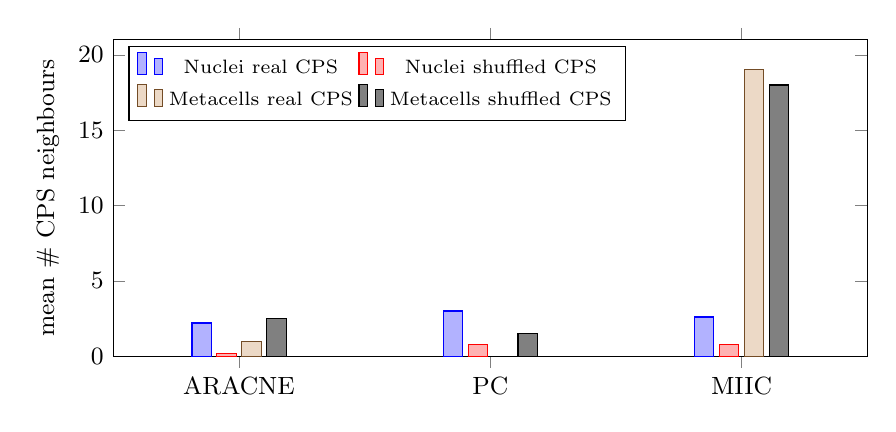
\begin{tikzpicture}
\begin{axis}[ybar, bar width=7pt, width=0.92\linewidth, height=5.6cm,
  symbolic x coords={ARACNE,PC,MIIC}, xtick=data,
  ylabel={mean \# CPS neighbours}, ymin=0, ymax=21,
  legend style={font=\scriptsize, at={(0.02,0.98)}, anchor=north west, legend columns=2},
  enlarge x limits=0.25, tick label style={font=\small}, ylabel style={font=\small}]
\addplot coordinates {(ARACNE,2.2) (PC,3.0) (MIIC,2.6)};
\addplot coordinates {(ARACNE,0.2) (PC,0.8) (MIIC,0.8)};
\addplot coordinates {(ARACNE,1) (PC,\pcCpsMeta) (MIIC,19)};   % PC value = \pcCpsMeta (macro in preamble)
\addplot coordinates {(ARACNE,2.5) (PC,1.5) (MIIC,18)};
\legend{Nuclei real CPS, Nuclei shuffled CPS, Metacells real CPS, Metacells shuffled CPS}
\end{axis}
\end{tikzpicture}
\caption{Number of CPS neighbours per method with real and shuffled CPS, for single nuclei (mean over five samples) and metacells. MIIC on metacells finds $\sim$18--19 neighbours with real \emph{and} shuffled CPS.\pcnote{}}\label{fig:cps}
\end{figure}

Over five independent samples of nuclei, a small set of genes remained robustly connected to CPS (Table~\ref{tab:stab}). \textbf{\gene{PTPRG}} was a CPS neighbour in 4/5 (ARACNE), 5/5 (PC) and 5/5 (MIIC) samples and never appeared with shuffled CPS. \gene{IQGAP2} was second (3/5, 4/5, 2/5), and \gene{BIN1} appeared in at most 2/5 samples, with a negative association. \gene{TGFBI}, found by all three methods in the first nucleus sample, appeared in only 1 of 15 runs afterwards and is therefore a sample-specific result. With random CPS, 0--2 spurious neighbours appeared per run (different genes each time), which gives a reference level of false links.

\begin{table}[ht]
\centering\small
\caption{Stability of CPS neighbours over five independent nucleus samples (number of samples in which the gene is a CPS neighbour).}\label{tab:stab}
\begin{tabular}{lccc}
\toprule
Gene & ARACNE & PC & MIIC\\
\midrule
\gene{PTPRG} & 4/5 & 5/5 & 5/5\\
\gene{IQGAP2} & 3/5 & 4/5 & 2/5\\
\gene{BIN1} (negative) & 2/5 & 1/5 & 2/5\\
\gene{TGFBI} & 0/5 & 1/5 & 0/5\\
\bottomrule
\end{tabular}
\end{table}

\subsection{Agreement with published work}
\gene{PTPRG}, \gene{TPRG1} and \gene{ZNF804A}, which we selected from the data, are among the DAM-supertype markers of Gabitto et al.\ (Fig.~6c), and in our networks they are connected to each other (\gene{TPRG1}--\gene{ZNF804A} and \gene{PTPRG}--\gene{ZNF804A} are consensus edges on metacells). That \gene{PTPRG} is also our robust CPS neighbour is consistent with the increase of the DAM supertype along CPS. We also reproduced the \gene{APOE}--\gene{CST3} link of the Adeoye MIC-M2 module (found by all three methods on both representations). In contrast, early-response genes of Gabitto (\gene{CSF1R}, \gene{C1QA/B}, \gene{IRF1/7}, Fc receptors) hardly correlated with CPS in our data (Spearman $\rho$ from $-0.2$ to $+0.17$). Genes increasing with CPS both in the papers and in our data but absent from our set include \gene{CTSD} ($\rho\approx+0.33$), \gene{NHSL1}, \gene{TANC2}, \gene{CADM1}, \gene{WIPF3}, \gene{MITF}, \gene{STARD13} and \gene{CD81}.

% =========================================================================
\section{Discussion}
\textbf{Which genes are directly linked to pathology?} Only \gene{PTPRG} was a reproducible direct neighbour of CPS across methods and samples; \gene{IQGAP2} and \gene{BIN1} are weaker candidates. This is a modest result, but a credible one: it is consistent with the DAM marker annotation, was never produced by shuffled CPS, and appears with the three methods, which rely on different assumptions. Because \gene{PTPRG} was selected as a data-driven marker of reactive microglia and not by its association with CPS, this finding is not circular. Most other genes (for example \gene{APOE}, \gene{CD74}, \gene{C1QA/B}) are tightly connected to each other, which suggests that their relation to disease is better described as the activity of a state (a reactive programme) than as individual direct effects.

\textbf{Metacells are a double-edged tool.} Aggregation recovered clean and biologically plausible gene--gene networks that single nuclei could not (many links vanished in nuclei because of zeros). But for a donor-level variable such as CPS, the same aggregation removes within-donor noise and leaves differences between people as the dominant signal. MIIC, which detects any statistical dependence and not only monotone trends, then connects CPS to everything that distinguishes donors. Without the shuffling control we would have reported 18 ``CPS-linked genes'' that include many genuine disease-response genes (\gene{APOE}, \gene{SPP1}, \gene{CD74}) and would have found a plausible biological story for them. The lesson is that a permutation control that preserves the donor structure should be standard for network inference with donor-level variables. In practice there are only $\sim$81--83 independent observations for CPS, not $\sim$1{,}000.

\textbf{Limitations.} (i) Most PC edges had conflicting orientations, so PC was used only for the presence of edges. (ii) A single CPS node captures monotone changes, whereas Gabitto et al.\ describe early rise followed by a plateau for many genes; such non-linear patterns are blurred, and this likely explains why early-response genes did not connect to CPS. (iii) The result depends on the choice of 48 genes out of 36{,}601. (iv) Edges are statistical associations, not causal claims; orientations from PC and MIIC are hypotheses. (v) The two data representations use different samples (12 nuclei per donor), and different random draws gave different weak edges, so only edges stable across samples should be trusted.

% =========================================================================
\section{Future work}
We plan to (1) analyse two alternative gene sets that we have already built and run: a ``literature'' set (genes from Gabitto Fig.~6 and Adeoye Fig.~8, $\sim$70 genes) and a ``data only'' set with the genes that vary most \emph{between metacells of the same donor}, which should select cell-state programmes rather than person-to-person differences; (2) replace the single CPS node by representations that capture early and non-linear changes (for example discretised CPS stages, or the DAM-supertype proportion per donor); (3) include donor-level covariates (age, sex, \emph{APOE} genotype) as network variables or adjust for them; (4) include the candidates \gene{CTSD}, \gene{CD81} and \gene{MITF}; and (5) validate \gene{PTPRG}--CPS in other SEA-AD regions or in an independent cohort.

% =========================================================================
\begin{thebibliography}{99}\small
\bibitem{Gabitto2024} Gabitto, M.I., Travaglini, K.J., Rachleff, V.M., et al.\ Integrated multimodal cell atlas of Alzheimer's disease. \emph{Nature Neuroscience} 27(12):2366--2383 (2024). doi:10.1038/s41593-024-01774-5
\bibitem{Hawrylycz2024} Hawrylycz, M., Kaplan, E.S., Travaglini, K.J., et al.\ SEA-AD is a multimodal cellular atlas and resource for Alzheimer's disease. \emph{Nature Aging} 4(10):1331--1334 (2024). doi:10.1038/s43587-024-00719-8
\bibitem{Adeoye2025} Adeoye, T., Shah, S.I., Ullah, G.\ Systematic analysis of biological processes reveals gene co-expression modules driving pathway dysregulation in Alzheimer's disease. \emph{Aging and Disease} 16(3) (2025); published online 21 June 2024. doi:10.14336/AD.2024.0429
\bibitem{Margolin2006} Margolin, A.A.\ et al.\ ARACNE: an algorithm for the reconstruction of gene regulatory networks in a mammalian cellular context. \emph{BMC Bioinformatics} 7(Suppl 1):S7 (2006).
\bibitem{Spirtes2000} Spirtes, P., Glymour, C., Scheines, R. \emph{Causation, Prediction, and Search}, 2nd ed. MIT Press (2000).
\bibitem{Verny2017} Verny, L., Sella, N., Affeldt, S., Singh, P.P., Isambert, H.\ Learning causal networks with latent variables from multivariate information in genomic data. \emph{PLoS Computational Biology} 13(10):e1005662 (2017).
\bibitem{Cabeli2020} Cabeli, V.\ et al.\ Learning clinical networks from medical records based on information estimates in mixed-type data. \emph{PLoS Computational Biology} 16(5):e1007866 (2020).
\bibitem{Baran2019} Baran, Y.\ et al.\ MetaCell: analysis of single-cell RNA-seq data using k-nn graph partitions. \emph{Genome Biology} 20:206 (2019).
\bibitem{Morabito2023} Morabito, S.\ et al.\ hdWGCNA identifies co-expression networks in high-dimensional transcriptomics data. \emph{Cell Reports Methods} 3:100498 (2023).
\bibitem{SEAAD} SEA-AD data: Allen Institute for Brain Science, immune-cell dataset (June 2026 release) and CPS table (\texttt{sea-ad\_global\_and\_local\_cps\_050126.xlsx}); donor metadata description (\texttt{sea-ad\_donorindex\_dataelementbriefdescriptions\_063026.pdf}).
\bibitem{Course} RESYS course materials: lectures on network reconstruction (ARACNE, PC, MIIC).
\end{thebibliography}

\end{document}
